\documentclass{amsart}

% I  moved all the document specific preamble stuff here so the top of this document doesn't get messy
\usepackage[english]{babel}
\usepackage{csquotes}
\usepackage[sortcites=true, sorting=nyt, backend=biber]{biblatex}

\usepackage[colorlinks=true,
pdfstartview=FitV, linkcolor=blue, citecolor=olive,
urlcolor=cyan]{hyperref}
\usepackage{xcolor, soul} %Package to insert links, citations, etc.

\usepackage{amsmath, amsthm, amssymb, mathtools}
\usepackage{graphicx} % Required for inserting images
\usepackage{geometry}
\usepackage{multicol}
\usepackage{tabularx}
\usepackage{changepage}
\usepackage[T1]{fontenc}
\usepackage{tikz}
\usepackage{listings} % Used for inserting code snippets
\usepackage{comment}
\usepackage{setspace}
\usepackage{todonotes}
\usepackage{tcolorbox} % used for drawing boxes around paragraphs so that notes are easier to identify

\usepackage{enumitem}
\usepackage{listings} % Used for including code snippets

\geometry{letterpaper, portrait, margin=2in}%1in}

\graphicspath{{Journal_Figures}}

\definecolor{myorange}{HTML}{ff7f00} % Defines the color of the box around text for tcolorbox

%https://osl.ugr.es/CTAN/macros/latex/contrib/tcolorbox/tcolorbox.pdf
\tcbuselibrary{breakable}
\tcbset{%any default parameters
	width=0.7\textwidth,
	halign=justify,
	center,
	breakable,
	colback=myorange    
}

% This controls how the code snippets are typset
\lstset{
	basicstyle=\ttfamily,
	columns=fullflexible,
	frame=single,
	breaklines=true,
	postbreak=\mbox{\textcolor{red}{$\hookrightarrow$}}\space
}

\lstset{language=Octave}


\newtheorem{theorem}{Theorem}[section]
\newtheorem{lemma}[theorem]{Lemma}

\theoremstyle{definition}
\newtheorem{definition}{Definition}[section]
\newtheorem*{example*}{Example}
\newtheorem{example}{Example}


\theoremstyle{remark}
\newtheorem{remark}{Remark}

\newlist{eqlist}{enumerate}{2}
\setlist[eqlist]{label=(\roman*), before=\raggedright}

% Nice way to make notes for myself
\newcommand{\William}[1]{\textcolor{red}{[William] #1}}

% Some nice math macros
\newcommand{\set}[1]{\left\{#1\right\}}
\newcommand*\diff{\mathop{}\!\mathrm{d}} % Changes the font of the differential d when writing dx or similar
\renewcommand{\st}{\colon} % renews the st command that is usually provided by soul to strike through
\newcommand{\N}{\mathbb{N}}
\newcommand{\R}{\mathbb{R}}
\newcommand{\Z}{\mathbb{Z}}
\newcommand{\Q}{\mathbb{Q}}
\newcommand{\RP}{\mathbb{RP}}
\newcommand{\Hyp}{\mathbb{H}}
\newcommand{\T}{\mathcal{T}}

\newcommand{\der}{\mathsf{d}}
\newcommand{\crossratio}[1]{\operatorname{CR}\left[#1\right]}

\newcommand{\metricd}{\operatorname{d}}

% Makes a todo list environment to make nice todo lists for things that would need to be shown
\newlist{todolist}{itemize}{2}
\setlist[todolist]{label=$\square$}

\newcommand{\inquotes}[1]{``#1''}

\newcommand{\close}[1]{\overline{#1}}

\newcommand{\wrt}{\text{w.r.t. }}
\newcommand{\proj}[1]{\pi\left(#1\right)}

\frenchspacing
%\doublespacing

\newenvironment{summary}{
	\hfill \break 
	\begin{center}
		\textbf{Summary:}
	\end{center}
	\begin{adjustwidth}{0.5in}{0.5in}
		
	
}{
\end{adjustwidth}
\bigskip
}

\usetikzlibrary{intersections}

\tikzset{
	convexset/.style = {line width = 0.75 pt, fill = white},
	ext/.style = {circle, inner sep=0pt, minimum size=2pt, fill=black},
	segment/.style = {line width = 0.75 pt}
}





 

% Resource Locations
\graphicspath{{Journal_Figures}}
\bibliography{meeting_journal_references.bib}

\title{Visualizing the Manhattan curve --- Journal}
\author{William Clampitt and Giuseppe Martone}
\date{November 2024}


\begin{document}

\begin{abstract}
    This notebook will serve as a research journal for William's master thesis project
\end{abstract}

\maketitle
\tableofcontents


\section{November 19, 2024}
\subsection{Meeting notes}
\subsubsection{Counting Problems}
	Gauss estimated that the distribution of prime numbers was 
	\begin{equation*}
		\# \set{p \in P \st p \leq T} \sim \frac{T}{\ln T} 
	\end{equation*}
	
	These type of counting problems are common in fields such as Geometry, Topology, and Dynamical Systems. 
	
	Typically, in this context
	\begin{equation*}
		\# \set{ a \in A \st a \leq T} \sim \text{ exponential in } T
	\end{equation*}
	
	\subsubsection*{Topoligical Entropy}
	Typically, topological entropy is calcualted with the below formula:
	\begin{equation*}
		h_{\text{top}}(A) = \lim_{T \to \infty} \frac{1}{T} \ln \# \set{a \in A \st a \leq T}
	\end{equation*}
	
	\begin{example*}
		\begin{equation*}
			h_{\text{top}}(\N) = 0
		\end{equation*}
	\end{example*}
	
	\subsubsection*{Hilbert Metric First Glance}
	
	\begin{figure}[h]
		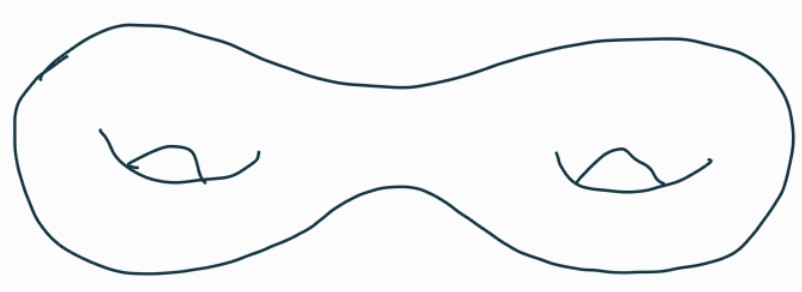
\includegraphics[width=0.5\linewidth]{g2_torus}
		\label{fig:g2_torus}
		\caption{Hyperbolic structure (locally looks like $\mathbb{H}^2$)}
	\end{figure}
	
	\begin{enumerate}
		\item You need a hyperbolic structure on $S$, call it  $p$.
		\item The set of closed loops (discrete)
		\begin{itemize}
			\item Each closed loop has a length \wrt the hyperbolic structure (number $> 0$)
		\end{itemize}
	\end{enumerate}
	
	We will denote the length of the curve $c$ as $l_p(c)$ \wrt $p \in \R$ where $p > 0$.
	\begin{equation*}
		\# \set{c \st l_p(c) < T} \sim \frac{e^T}{T}
	\end{equation*}
	\begin{remark}
		This was shown by Huber Marpulis \William{Is this person the same as Grigory Margulis? Maybe I wrote the name down wrong when I was taking notes.}
	\end{remark}
	
	\subsubsection*{Origin of Program Matrices}
	
	The three matrices in the first program are representing a relfection accross the three distinct edges of the triangles that are formed when we stretch the holes of our pants to the boundary of our hyperbolic space. 
	
	
\subsection{Post-meeting notes}

\subsubsection{Counting Problems}

\begin{example*}
	The distribution of prime numbers. In 1792 Gauss proposed that
	\begin{equation*}
		\pi(n) \sim \frac{n}{\ln n}
	\end{equation*}
	
	but was later refined to 
	\begin{equation*}
		\pi(n) \sim \text{Li}(n),
	\end{equation*}
	
	where
	\begin{equation*}
		\text{Li}(n) = \int_{2}^{n} \frac{\diff x}{\ln x}
	\end{equation*}\cite{wolfram_prime_num_theorem}
\end{example*}


\section{December 3, 2024}
\subsection{Meeting notes}

\begin{summary}
	In this meeting we discussed the problems that I encountered with my program. In summary, my program is using up too much system memory of the computer. This results in the program crashing which prematurely halts the calculation of the words of our alphabet. Because I was not incrementally storing the already computed matrices, the program would not yeild any results if it crashed. 
\end{summary}



\subsubsection*{Potential Solutions to Problem}
I think one way that might be good to reduce the system memory useage of my program would be to store the words of length $n$ in a file, then use those words to generate the words of length $n + 1$. The words of length $n$ would then be unloaded from system memory. After the words of length $n$ are unloaded, we can use the words of length $n + 1$ to calculated the words of length $n + 2$ and so on. 

\subsection{Post-meeting notes}

I am attempting to rewrite my current program using Octave while also implimenting my idea about iteratively saving the words of length $n$ each time so that I do not have to store the entirety of the list in system memory at one time. After this is done, the list will need to be sifted through to remove duplicates matrices.  

\newpage
\printbibliography

\end{document}
